%%%%%%%%%%%%%%%%%%%%%%%%%%%%%%%%%%%%%%%%%
% Imperial Placement Report Template 
% LaTeX Template
% Version 1.0 (28/06/16)
%%%%%%%%%%%%%%%%%%%%%%%%%%%%%%%%	%%%%%%%%%
%----------------------------------------------------------------------------------------
%	PACKAGES AND OTHER DOCUMENT CONFIGURATIONS
%----------------------------------------------------------------------------------------

\documentclass[a4paper]{article}
\usepackage[english]{babel}
\usepackage[utf8x]{inputenc}
\usepackage{amsmath}
\usepackage{graphicx}
\usepackage[colorinlistoftodos]{todonotes}
\usepackage[toc,page]{appendix}
\usepackage[T1]{fontenc}
\usepackage[a4paper,top=2cm,bottom=2cm,left=2.5cm,right=2.5cm,marginparwidth=1.75cm]{geometry}

\begin{document}

\begin{titlepage}

\newcommand{\HRule}{\rule{\linewidth}{0.5mm}} % Defines a new command for the horizontal lines, change thickness here
\setlength{\topmargin}{0in}
\center % Center everything on the page
 
 
 \begin{minipage}{0.4\textwidth}
\begin{flushleft} \large
\hspace*{-0.5cm}
\end{flushleft}
\end{minipage}
~
\begin{minipage}{0.5\textwidth}
\begin{flushright} \large
\hspace*{2cm}
% \includegraphics[scale=0.4]{company.png}\\
\end{flushright}
\end{minipage}\\[1cm]
%----------------------------------------------------------------------------------------
%	HEADING SECTIONS
%----------------------------------------------------------------------------------------

\textsc{\LARGE Imperial College of Science, Technology and Medicine}\\[1.5cm] % Name of your university/college
\textsc{\Large Department of Computing}\\[0.5cm] % Major heading such as course name

%----------------------------------------------------------------------------------------
%	TITLE SECTION
%----------------------------------------------------------------------------------------

\HRule \\[0.4cm]
{ \huge \bfseries BeatIt}\\[0.4cm] % Title of your document
\HRule \\[1cm]
 
%----------------------------------------------------------------------------------------
%	AUTHOR SECTION
%----------------------------------------------------------------------------------------

\textsc{{\large
\textbf{Group 11} \\
Yoram \textsc{Boccia}, \\
Justin \textsc{Chong}, \\ 
Halite \textsc{Abudureyimu}, \\
Hadrian \textsc{Lim} }}\\[0.5cm]

%----------------------------------------------------------------------------------------
%	DATE SECTION
%----------------------------------------------------------------------------------------

{\large \today}\\[0.5cm] % Date, change the \today to a set date if you want to be precise


\vfill % Fill the rest of the page with whitespace

\end{titlepage}

\newpage

\section{Group Work Allocation}
At the beginning of this project, the group was split into 2 subgroups:\\ \\
Halite Abudureyimu and Yoram Boccia co-worked on Part 1: the emulator. Halite designed the structure of the emulator. He coded the emulate.c, pipeline.c and emuexecute.c files. Meanwhile, Yoram coded the arm11io.c, emudecode.c, operation.c files. Communication was really good between the two. Both of them debugged, cleaned and reorganized the files together.
\\\\
Justin Chong and Hadrian Lim co-worked on the second part: the assembler. Justin outlined the structure of the assembler. He implemented the assembler IO and the logic behind parsing string tokens and arranging the bitcodes. He also implemented a dynamic memory access structure to maintain minimal memory cost and reduce input-output overhead. Hadrian Lim implemented key utility functions such as the lookup, extractBits functions. He also helped encode and decode the binary instructions. Debugging and testing was done together by Hadrian and Justin.
\\\\
We all worked together on the third part and for the extension we split the work again into two parts. Yoram Boccia and Halite Abudureyimu worked on the controller, whilst Justin Chong and Hadrian Lim implemented the game and its structure.  
\\\\
While we were progressing with the project, we used GitLab to combine our work. We did so by pushing up the codes to our own branches, where the group leader was then responsible for merging and maintaining the different codes accordingly.

\section{Opinions about Group Working}
\textbf{Halite:}\\
I think we are cooperating with each other really well. Yoram and I did the first part. During the working period, we communicated with each other alot. Especially during the debugging, we took turns operating the computer every two hours, while the other assisted from the side. This was really helpful for our efficiency since debugging is a really overwhelming job. In order to work together more effectively and delightfully, We hang out together beyond the working time, like playing football.\\
\\
\textbf{Yoram:}\\
I believe that our group is really motivated and we really communicated in an efficient way. We communicated right from the the beginning and split the work between us.
Halite and I worked really well on the emulator part. We planned the work together before starting coding out own part. Debugging was the best part because together we understood our final code and we wrote tests for every file before debugging the whole emulator. For the next tasks I believe we should continue in the same way we are already doing, but maybe hanging out more together to rest a little bit from the project.
\\\\
\textbf{Justin:}\\
Our team were quick to decide on splitting the work, and Hadrian and I were tasked with tackling the assembler. Overall, I think we had good team synergy. Parts that I found confusing, such as the move command register shifting, and the rotates for immediate addressing, were only possible to tackle with the help of my teammates. I think we are quite productive as a team, thanks to our constant communication and structured work schedules. Overall, we might need to get ready to modularise the projects even more as we move to part 3 and 4. Part 3 and 4 cannot be done concurrently, and are projected to be much harder than the first two parts. Overall, we would probably need to get to know each other a little more, to see where each individual is suited to do what tasks.\\
\\
\textbf{Hadrian:}\\
Communication within the group has been smooth so far. The group has been able to meet the deadlines that we agreed upon so far. Criticism towards each other's work has been constructive and well received. We can easily approach members of our team if we have any queries regarding the C language. All in all, the team has a healthy dynamic that boosts productivity. For the future parts (III and IV), we will have to seperate the work initially, such that each of us do not depend on each other's code. If we depend too much on each other's implementations, we might end up having to wait for each other and slow down individual development.

\section{Details About Emulator}
There were several keywords that helped us to decompose the whole emulator, such as: $read and write$, $pipeline$, $alu$, $shifter$, $execute$, $decode$ and $fetch$. The spec helped us split the instructions into 4 main types. Thus, We used the keywords to structure the different files according to the respective instructions types. Then, Yoram and Halite discussed and confirmed over the details about the preconditions and postconditions of their own parts as following:
\\\\
\textbf{emulate.c:} the main functions is pretty straightforward: allocate memory to state, read binary, simulate the pipeline, and write out the result. So it calls $new\_state$ and $delete\_state$ in \textbf{emustruct.c}, $emuread$ and $emuwrite$ f in \textbf{arm11io.c}, and $pipeline\_circle$ functions in \textbf{pipeline.c}.
\\\\
\textbf{arm11io.c:} contains 2 major functions: $emuread$ and $emuwrite$. \textbf{emuread} read the binary file and convert the binary numbers into decimal form and save it into our "memory".
\textbf{emuwrite:} outputs the result of "registers" and "non-zero memory address".
\\\\
\textbf{pipeline.c} contains 4 major functions: $pipeline\_circle$, $execute$, $decode$, and $fetch$. The $pipeline\_circle$ uses the other 3 functions to simulate the process. $fetch$ get the instruction code from the "memory". $decode$ decomposes the fetched code into small parts according to 4 major instruction types by calling them in \textbf{emudecode.c}. Finally, $execute$ function passes the instruction and storage into 4 major instruction type execution coded in \textbf{emuexecute.c} .
\\\\
\textbf{emudecode.c} contains 4 major functions according to 4 different instruction types.
\\\\
\textbf{emuexecute.c} contains 4 major functions according to 4 different instruction types. And specifically, the $execute\_data\_processing$ function implements the instruction by putting elements into \textbf{alu} and \textbf{shifter}, which are combined in \textbf{operation.c}
\\\\
\textbf{operation.c:} contains all the operations coming from the alu and the shifter.
\\\\
\textbf{emudef.h:} contains all the definitions of constant number and enum types in our emulator project.
\\\\
\textbf{emustruct.h:} contains all the struct types we used in the project, such as State, Storage and Instructions, and the declaration of $new\_state$ and $delete\_state$ functions.

%\section{Usefull Skills for the Assembeler}
%Generally, knowledge in how the binary instructions will be decoded in the emulator helps in understanding the encoding for assembly instructions. As such, members working on the emulator could help provide valuable feedback on any misunderstandings regarding the assembler.
%\\\\
%Specifically in terms of implementation details, there are a few functions used in the emulator that we have found useful for the assembler. These are general functions that deal with bits manipulation. Examples of such functions include a function to logical shift right and a function to extract certain bits from a binary representation.

\section{Details About Assembler}
The Assembler can be split into two main loops, the first pass, and the second. In the first pass, the assembler builds the symbol table to be used for branching. It also initializes several parameters to be used in the second pass such as the number of instructions, etc.
\\\\
The second pass iterates through and dynamically parses each instruction string, by calling the $parseString$ function. Based on the instruction string, $parseString$ calls and returns the result from the corresponding parser in \textbf{parseData.c}. These results are binary instructions which are then stored in an array.
\\\\
The parsers in \textbf{parseData.c} produce binary instructions based on knowledge of the specific ARM instruction ($Data\ Processing$, $Multiply$, $Single\ Data\ Transfers$, and $Branching$). They work by populating an Instruction\_t with relevant parameters. It then builds a binary instruction by calling corresponding encoding functions in \textbf{assencode.c}.
\\\\
The data structures used throughout the assembler are as follows: The symbol table is stored as an array of $symbol$ structs. Each $symbol$ struct contains the label and it's corresponding line number. The instruction binary data is stored as an array of unsigned 32 bit integers.
\\\\
\textbf{assemble.c:} Entry point of the assembler, which defines the logic for the first and second passes. It handles line by line file IO and passes it into the first pass and second pass functions. The function then calls the $parseString$ function from \textbf{parseStr.c}, which return result is a binary instruction. It stores the resulting binary output into the $uint32\_t$ array, and writes it to the output file after parsing all instructions.
\\\\
\textbf{parseStr.c:} Identifies the assembly instruction via character matching of the input string. It then calls the corresponding function from \textbf{parseData.c} whilst passing in relevant parameters based on the input string (such as opcode).
\\\\
\textbf{parseData.c:} Takes in parameters and wraps it in the instruction struct, to be encoded into binary by \textbf{assencode.c}.
\\\\
\textbf{assencode.c:} This file contains code that will encode a binary instruction. More specifically, an instruction struct containing the relevant parameters (Rn, Operand2, etc.) will be passed in to the encoding functions. The encoding functions then utilises these parameters to encode a binary instruction.
\\\\
\textbf{strutils.c:} Contains several helper functions that helps string parsing. 

\section{Details about the Extension}
We decided to build and design a game using the C programming language and utilize the Raspberry Pi as a game controller. The game is a rhythm fighting game hybrid, where the player will control Michael Jackson to fight off thugs, to the tune and beats of famous MJ songs. MJ starts at the middle, and enemies will approach MJ from the left and right of the screen. The player then has to time his attacks to the left and right based on the rhythm of the song, in order to defeat enemies and score points. Control of the game is through five buttons on the Raspberry Pi, which will emulate keyboard inputs through BlueTooth. The aim of the game is using a control to play and have fun
\begin{figure}[h]
\centering
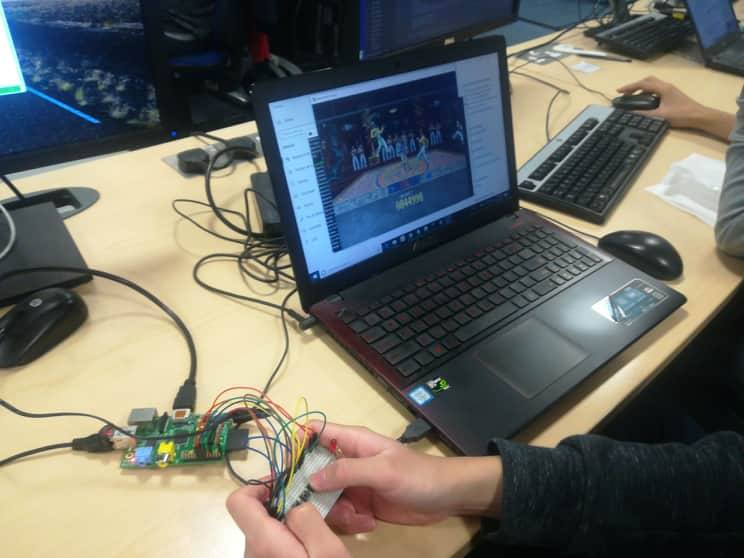
\includegraphics[width=0.6\textwidth]{game.jpg}
\caption{\label{fig:pi}This is an example of the game}
\end{figure}


\textbf{1.Abstract:}  Yoram and Halite did the controller part of our extension. In this part, we built software which allows the Raspberry Pi to function as a bluetooth keyboard emulator. The Raspberry Pi is connected to a breadboard which functions as our "Keyboard". If we pressed the buttons on our "Keyboard", we can control the action of our main character in our BEATIT game. For this part we followed the “Emulate a Bluetooth keyboard with the Raspberry Pi” tutorial and made relevant changes to it.
For the programming part, we choose the Python language to code our program. The language seems to be the most suitable for the task, as there are plenty of libraries we can use to build our controller in a really limited time. None of us have learned Python before, so we spent three days to learn the python’s syntax and useful functions.\\\\
Meanwhile, Justin and Hadrian built the game from scratch. In this section, we used X11lib and SDL2 as interface libraries for IO, and everything else was written from scratch. We built a render library that parses bitmap files into a 2D pixel array, does sprite logical processing and has several entry point functions to be used with X11lib to display the pixels onto the screen. We also built a gameloop library that includes separate libraries for the player, enemy, levels, gameState, menus and so on. The main game loop updates the game state and then renders the gamestate onto the screen.\\\\

\begin{figure}[h]
\centering
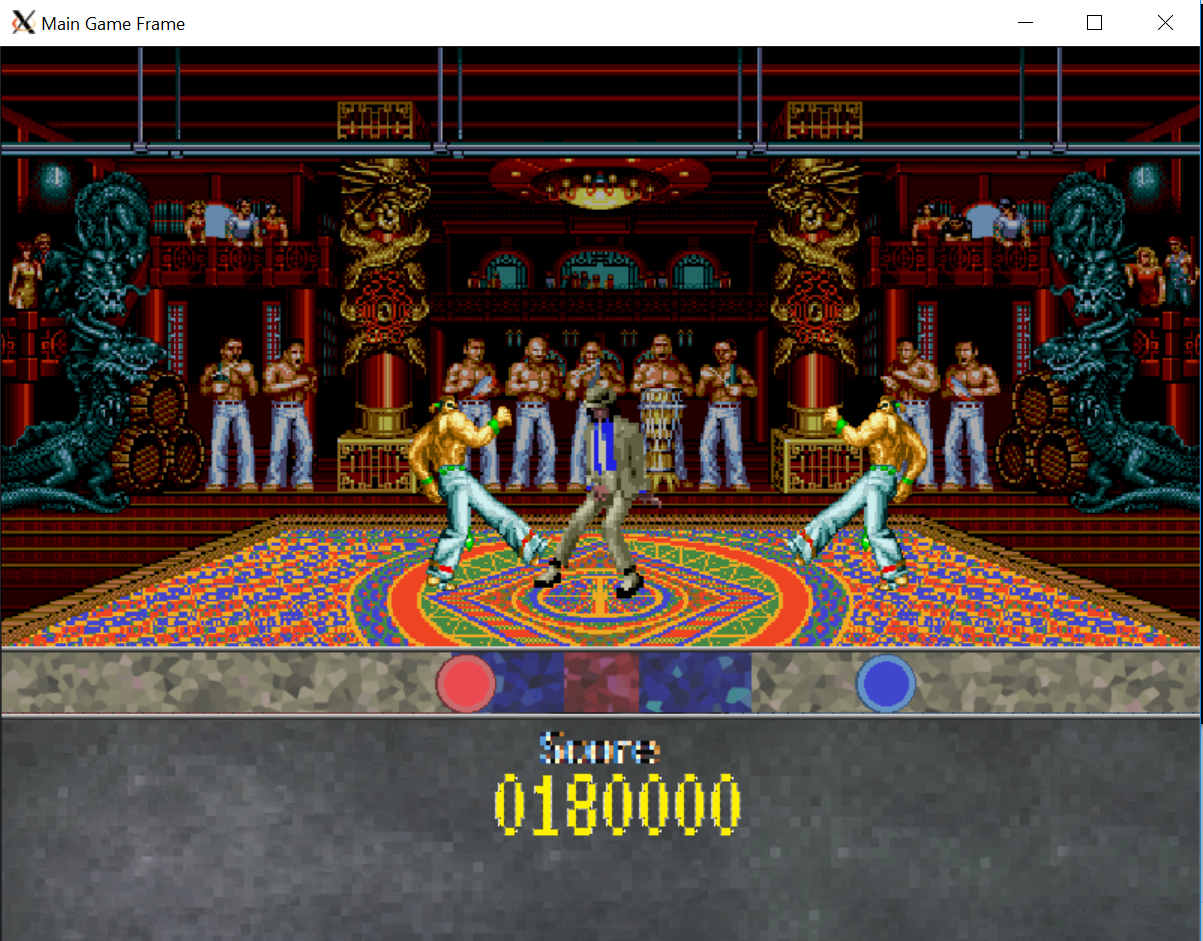
\includegraphics[width=0.6\textwidth]{game_graphics.png}
\caption{\label{fig:pi}This is a demonstration of the game screen}
\end{figure}


\setlength{\parindent}{0cm}
\textbf{2.Hardware:}\\\\
1) A Raspberry Pi with all necessary peripherals   \\\\
2) A USB Bluetooth dongle \\\\
3) A USB hub – if you want to use a keyboard and mouse at the same time as the Bluetooth dongle  \\\\
4) 5 button switches  (emulate A, S, E, Q, W respectively in Figure 1).  \\\\

\begin{figure} [h]
\centering
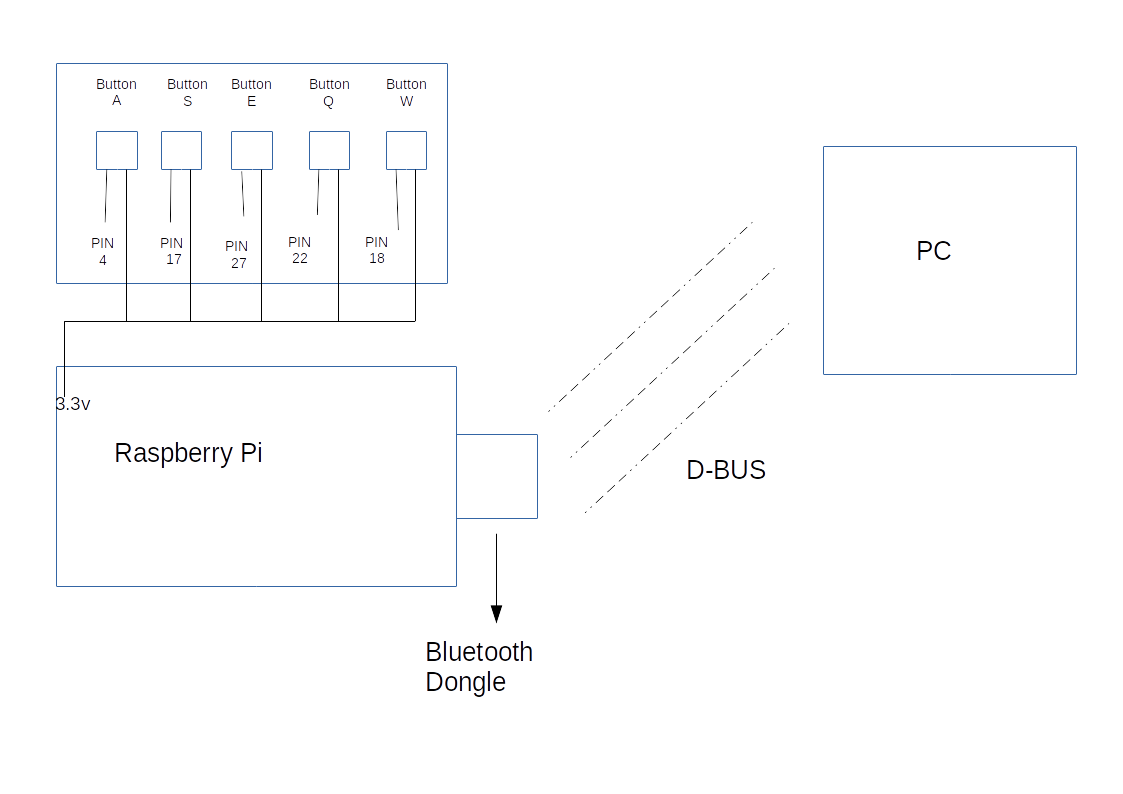
\includegraphics[width=0.6\textwidth]{pidemo.png}
\caption{\label{fig:pi}This is the demonstration of pi and PC connection}
\end{figure}


\setlength{\parindent}{0cm}
\textbf{3.Files:} \\\\
\underline{kb\_client.py:}\\
\quad  i) Connection between Pi and PC. We use bluetooth dongle as a connection device and D-Bus as the communication interface by using SDP(Service Discovery Protocol)
\\\\
ii) Gets the input from pi: We import RPi.GPIO library to setup and read our inputs. And use keymap.py file to convert our input into codes which is compatible to the D-BUS SDP format.
\\\\
iii) Sending the input:	this part is simple, after getting the correct sending format, simple use cinterrupt.send(str) to send our input to the server, and our pc would get the signal from it.
\\\\
\underline{keymap.py:} \\This file contains a dictionary mapping evdev keys to Bluetooth keys 
sendingstring.py and btkserver.py (We use the authors code, the details are in the references.)
\section{Design and Challenges/Problems}
At the beginning we thought it would be challenging to implement the extensions for this project because we had just one Raspberry Pi for four people in the group. 
Moreover, another issue to take in consideration was going to be the small amount of time we had for this project, after solving the first three parts. Hence, we planned first every detail of our extension and then we split the work between the four of us.
\\\\
\textbf{game logic:} When dealing with implementing the game logic, great care had to be taken to make any features extensible. For example, it might be tempting to utilise a one liner hack in order to achieve an outcome in the short term. However, we have noticed that this necessitates large refactorings in the future as the codebase grows larger.
\\\\
\textbf{rendering:} It was difficult to find an appropriate graphics library that could be light weight, support a multitude of platforms, whilst using the standard libraries (as we decided not to use libraries that aren't installed in lab machines). Eventually we managed to find and slightly modify an libX11 wrapper, that was very lightweight and supported simple input output detection. The bare bone nature of the library made it inefficient, which eventually led to the slowdown of the application on Lab computers, requiring us to optimize the rendering process. 
\\\\
\textbf{audio:} It was near impossible to find a C audio library that could handle cross platform file parsing and audio playback. We eventually decided to rely on the built in SDL2.
\section{Testing the Extension}
We split the work into two parts and we have tested both of them.
\\\\
\textbf{Controller:} After coding, we tried to connect our pi to different devices: Linux, Windows, Mac PCs and Android and IOS phones. The connection overall is stable and suitable for the above devices. The effect of pressing the buttons is stable, correct and always the same.
\\\\
After connecting the pi to the PC, The BEATIT game and all its functions work correctly.
We think that this way of testing our project is overall effective.
\section{Group reflection}
We worked really well together. From the beginning we communicated a lot. We understood the strengths of each member of the group and, accordingly, we split the different tasks throughout the implementation of the project. We started splitting the work since the beginning with the emulator and we found it very useful. Everyday, we would meet all together to explain the progresses and to plan the next tasks. We used git extensively for version control. Each of us worked on a different branch initially and then merged all the different parts together at a later stage. 
\\\\
We believe that we communicated in a very efficient way and that the way we split the work was very helpful. Every time we had to implement another task, we would first analyze everything and build up the structure of the project together. We made sure all of us understood what was going on and that what we wanted to make was doable in the available time. Only then did we actually start coding. We think that this planning really helped us a lot as we always finished the different tasks before the deadlines we planned for ourselves. Moreover, we also organized football matches and dinner together to create a friendly atmosphere in the group. This helped a lot because we dealt with each part of the project with enthusiasm. Every time one of us had problems, we would also work together to solve them.

\section{Individual reflection}
\textbf{Halite:}\\
I personally believe that this project is one of the greatest experience in my life. During this period, I learned lots of communication skills, programming cooperation techniques, as well as useful project developing knowledge. For example, I learned how to use GitLab and GitHub efficiently with my teammates. Also, I learned how the network connection works and what is D-Bus, SDP. Furthermore, I acquired some electrical components and circuits knowledge whilst working with Raspberry Pi. Regarding our team, none of us had much experience in a large scale programming group project before. However, we managed to develop a game and bluetooth keyboard in a really limited time. I think for a bunch of beginners it is not easy. All of the members worked hard, learned lots of new knowledge, and made really great contributions to the project. I want to thank the department for providing us with this opportunity and my teammates for being wonderful.
\\\\
\textbf{Yoram:}\\
I believe that we really worked proficiently together. I fitted in the group very well. I have never programmed in C before, as other members of my group, but all together we helped each other and we put a lot of effort in learning and in solving the different parts of the project. At the beginning I was a little bit scared because I did not know this programming language, but I was not the only one and I just had to work maybe harder at the beginning to learn it. Some of my strengths that I think really helped the group are the creativity, the fact that I want to have a clean and structured code, and the will to test every single function to be sure that everything works as we want.
I would not change anything we did as a group because we had an efficient communication and we have split the work in a proficient way. With different people I would create again the same friendly environment in order to work well together. I would analyze the tasks before starting to implement them, I would plan some deadlines to respect and I would continue to use Git to split the work and then merge it. 
\\\\
\textbf{Justin:}\\
I felt like the extension pushed our team to a new level. The amount of roadblocks we encountered skyrocketed, and the fact that all of the development being so interlinked required us to work closely with each other to ensure there will be no bottlenecks in development. This really pushed our team to bond closer as we pushed through late nights together. I feel like I've learned a lot about group project planning, and compartmentalizing our workload, and I'm very happy on how we managed to work very efficiently with minimal stalling from the lack of teamwork. I feel that in the future, I would probably spend a little more time laying out and agreeing on a clear project style, so that we can avoid spending time refactoring and reformatting code that has already been written. Overall, I'm impressed of how well the work-flow turned out.\\
\\
\textbf{Hadrian:}\\
Compared to when we were dealing with the assembler and emulator, I feel like the group has improved in terms of work distribution and having a smooth work flow. There were seldom, if any, bottlenecks in the development process for our extension. The direction was set from the initial stage and everyone was on the same page throughout the project. Specific to the extension, I feel like my knowledge in game development has helped made this project smoother. This is in terms of knowing common game development practices that helped form the skeleton of the game logic. There were certain minor issues that we would do differently when working in future group projects. An example would be to agree upon a certain style of code. Simple things such as number of spaces for indents and having camelCase variables instead of underscoring drained us of a couple hours in refactoring. Hence, it would be beneficial in future group projects to agree upon certain practices before coding.

\section{References:}
https://www.gadgetdaily.xyz/emulate-a-bluetooth-keyboard-with-the-raspberry-pi/\\
http://mlabviet2016.blogspot.com/2017/09/make-raspberry-pi3-as-emulator.html\\
https://en.wikipedia.or/wiki/Session\_Description\_Protocol\\
https://impythonist.wordpress.com/2014/02/01/emulate-a-bluetooth-keyboard-with-the-raspberry-pi/



\end{document}
